\documentclass[12pt,letterpaper]{article}

\usepackage[margin=1in]{geometry}
\usepackage{times}
\usepackage[utf8]{inputenc}
\usepackage[T1]{fontenc}
\usepackage{amsmath}
\usepackage{amssymb}
\usepackage{graphicx}
\usepackage{booktabs}
\usepackage{url}
\usepackage{xurl}
\usepackage[hidelinks]{hyperref}
\usepackage{setspace}
\usepackage{fancyhdr}
\usepackage{tocloft}
\usepackage{microtype}
\usepackage{float}
\sloppy

\renewcommand{\figurename}{Figura}
\renewcommand{\tablename}{Tabla}
\renewcommand{\contentsname}{\'Indice}

\setlength{\headheight}{15pt}
\pagestyle{fancy}
\fancyhf{}
\fancyhead[R]{\thepage}
\renewcommand{\headrulewidth}{0pt}

\begin{document}

% ---------------------------------------------------------------
% Car\'atula
% ---------------------------------------------------------------
\begin{titlepage}
\centering

\includegraphics[width=0.28\linewidth]{images/logo_ues.png}\par
\vspace{0.5cm}
{\large UNIVERSIDAD DE EL SALVADOR\par}
{\large FACULTAD DE INGENIER\'IA Y ARQUITECTURA\par}
{\large ESCUELA DE INGENIER\'IA DE SISTEMAS INFORM\'ATICOS\par}
\vspace{2.5cm}
{\Large\bfseries Clasificaci\'on de Enfermedades, Plagas y Deficiencias Nutricionales en Hojas de Ma\'iz mediante Modelos Convolucionales Ligeros: Recolecci\'on de Datos, EDA y Baselines\par}
\vspace{1cm}
{\large Etapa 1 \par}
\vspace{2.5cm}
{\large\bfseries Integrantes:\par}
\vspace{0.3cm}
{\large Josias Abner Rivas Fuentes -- RF20010 \par}
{\large David Alejandro Deras Cerros -- DC19019 \par}
{\large Elmer Edenilson Rosales Molina -- RM20001 \par}
\vfill
{\large San Salvador, El Salvador \par}
{\large \today \par}
\end{titlepage}

\newpage
\tableofcontents
\newpage

\doublespacing

\section*{Resumen}
\addcontentsline{toc}{section}{Resumen}
Este trabajo presenta la Etapa~1 de un sistema de clasificaci\'on de enfermedades foliares, plagas y deficiencias nutricionales en cultivos de ma\'iz mediante \textit{deep learning}, orientado a inferencia completamente offline en dispositivos m\'oviles de gama media/baja. Se documenta la recolecci\'on y limpieza de un conjunto de datos consolidado de 31~623 im\'agenes en 9 clases procedentes de 6 fuentes p\'ublicas, un an\'alisis exploratorio que identifica un desbalance de clases de hasta 32.9$\times$ y sesgos de dominio laboratorio/campo, el pipeline de preprocesamiento y balanceo, y la comparaci\'on de tres arquitecturas convolucionales ligeras preentrenadas en ImageNet (ShuffleNetV2-x1.0, EfficientNet-B0 y EfficientNet-Lite0) sobre las 9 clases del dataset con un tope de 1~500 im\'agenes por clase (10~020 im\'agenes en total). EfficientNet-B0 obtiene el mejor macro-F1 en prueba (0.9146), seguido por ShuffleNetV2-x1.0 (0.9030) y EfficientNet-Lite0 (0.8951). Los tres superan la meta de macro-F1 $\geq0.85$. Un an\'alisis de la matriz de confusi\'on revela dos cl\'usteres de error: las deficiencias nutricionales (N/P/K), donde \texttt{potassium\_deficiency} concentra el mayor n\'umero de confusiones con F1 de 0.49--0.62, y las lesiones foliares (\texttt{gray\_leaf\_spot} $\leftrightarrow$ \texttt{northern\_corn\_leaf\_blight}). Un an\'alisis con LIME sobre casos individuales muestra que los modelos concentran la atenci\'on en tejido foliar en aciertos.

\noindent\textbf{Palabras clave:} clasificaci\'on de enfermedades foliares, ma\'iz, redes neuronales convolucionales, transfer learning, LIME, dispositivos m\'oviles

\newpage

\section{Introducci\'on}

La agricultura representa el 5.6\% del PIB de El Salvador y es sustento de m\'as de 2 millones de personas en zonas rurales; el 82.1\% de los productores son peque\~nos agricultores, muchos a nivel de subsistencia. El ma\'iz, cultivo principal, es vulnerable a enfermedades foliares, plagas y deficiencias nutricionales que, sin detecci\'on temprana, pueden destruir hasta el 70\% de la cosecha; la cosecha nacional cay\'o un tercio entre 2021 y 2023.

En zonas rurales el acceso a asistencia t\'ecnica agr\'icola es limitado --- una condici\'on de infraestructura del sector, no un juicio sobre el conocimiento del agricultor. Como consecuencia, el diagn\'ostico depende con frecuencia de la experiencia emp\'irica de quien cultiva, lo que puede favorecer detecciones tard\'ias y p\'erdidas econ\'omicas. Este proyecto no busca reemplazar la asistencia t\'ecnica ni al extensionista agr\'icola, sino ofrecer una \textbf{herramienta de apoyo} que permita detectar tempranamente una condici\'on foliar y orientar sobre pr\'oximos pasos, de forma complementaria al conocimiento existente del agricultor.

La soluci\'on propuesta es un modelo de clasificaci\'on de im\'agenes liviano, capaz de ejecutarse completamente offline en un dispositivo Android de gama media/baja (${\geq}$4~GB RAM, Snapdragon serie 6xx o equivalente). El agricultor captura o sube una foto de una hoja de ma\'iz y la aplicaci\'on responde con la clase m\'as probable, su porcentaje de confianza y consejos de manejo asociados. El modelo objetivo no supera los 20~MB y mantiene una latencia de inferencia ${\leq}300$~ms por imagen, empleando cuantizaci\'on INT8 y un runtime m\'ovil (p.~ej.\ TensorFlow Lite u ONNX Runtime Mobile).

Esta primera etapa cubre la recolecci\'on y documentaci\'on del dataset, el an\'alisis exploratorio de datos, el pipeline de preprocesamiento y balanceo, y la comparaci\'on de tres arquitecturas candidatas como \textit{baseline} sobre las 9 clases del dataset, antes de comprometer el entrenamiento final y el despliegue m\'ovil.

\section{Descripci\'on del Dataset}

El dataset consolidado en \texttt{clean/} re\'une \textbf{31~623 im\'agenes} en \textbf{9 clases}, integradas y depuradas a partir de 6 fuentes p\'ublicas (Tabla~\ref{tab:sources}). Cada imagen queda etiquetada por entorno de captura: \texttt{lab} (fondo controlado) o \texttt{real} (campo abierto).

\begin{table}[H]
\caption{Fuentes de datos evaluadas y su licencia}
\label{tab:sources}
\centering
\small
\begin{singlespace}
\begin{tabular}{p{2.3cm}p{1.6cm}p{2.6cm}}
\toprule
\textbf{Fuente} & \textbf{Dominio} & \textbf{Licencia} \\
\midrule
Maize in Field Dataset & Campo real & CC BY-NC-SA 4.0 \\
Maize Diseases & Lab + campo & CC BY-NC-SA 4.0 \\
CropDG Unified Multi-Domain & Multi-dominio & CC BY-NC-SA 4.0 \\
Maize / Beans / Tomatoes -- \'Africa & Campo real & Apache 2.0 + CC \\
Maize Nutrient Deficiency & Campo real & CC BY 4.0 \\
Corn Leaf -- Roboflow & Campo real & CC BY 4.0 \\
\bottomrule
\end{tabular}
\end{singlespace}
\end{table}

Dos fuentes adicionales evaluadas fueron descartadas: \textit{Corn Leaf Diseases} (MIT), porque solo distribuye im\'agenes ya aumentadas sint\'eticamente sin conservar los originales; y \textit{Multicrop Disease} (licencia no especificada), por mezclar sin metadatos im\'agenes preprocesadas, de laboratorio y de campo, lo que impide separarlas de forma confiable.

Durante la limpieza se detectaron duplicados \emph{entre} fuentes distintas mediante hash perceptual (pHash, \texttt{imagededup}), eliminando \textbf{8~538 im\'agenes} agrupadas en \textbf{8~050 grupos} -- principalmente entre las fuentes \textit{maize\_desease} ($\sim$6~508) y \textit{multi\_desease} ($\sim$1~980). Sin esta depuraci\'on, im\'agenes id\'enticas habr\'ian aparecido en train y validaci\'on, inflando artificialmente las m\'etricas por fuga de datos.

La Tabla~\ref{tab:classes} muestra la composici\'on final por clase y entorno.

\begin{table}[H]
\caption{Composici\'on del dataset limpio por clase}
\label{tab:classes}
\centering
\small
\begin{singlespace}
\begin{tabular}{lrrr}
\toprule
\textbf{Clase} & \textbf{Lab} & \textbf{Real} & \textbf{Total} \\
\midrule
healthy & 0 & 8~744 & 8~744 \\
northern\_corn\_leaf\_blight & 888 & 5~942 & 6~830 \\
lethal\_necrosis & 0 & 6~415 & 6~415 \\
fall\_armyworm & 0 & 4~858 & 4~858 \\
common\_rust & 2~150 & 106 & 2~256 \\
gray\_leaf\_spot & 513 & 606 & 1~119 \\
phosphorus\_deficiency & 0 & 612 & 612 \\
nitrogen\_deficiency & 0 & 523 & 523 \\
potassium\_deficiency & 0 & 266 & 266 \\
\midrule
\textbf{Total} & \textbf{3~551} & \textbf{28~072} & \textbf{31~623} \\
\bottomrule
\end{tabular}
\end{singlespace}
\end{table}

\section{An\'alisis Exploratorio de Datos}

El EDA completo, reproducible en \texttt{notebooks/01\_eda.ipynb}, identific\'o cinco riesgos principales para el entrenamiento.

\textbf{Desbalance de clases.} La clase \texttt{healthy} (8~744 im\'agenes) supera en \textbf{32.9$\times$} a \texttt{potassium\_deficiency} (266); ver Figura~\ref{fig:dist}. Este cociente motiv\'o el uso de \texttt{WeightedRandomSampler} combinado con augmentation extendido en las clases minoritarias.

\begin{figure}[H]
\centering
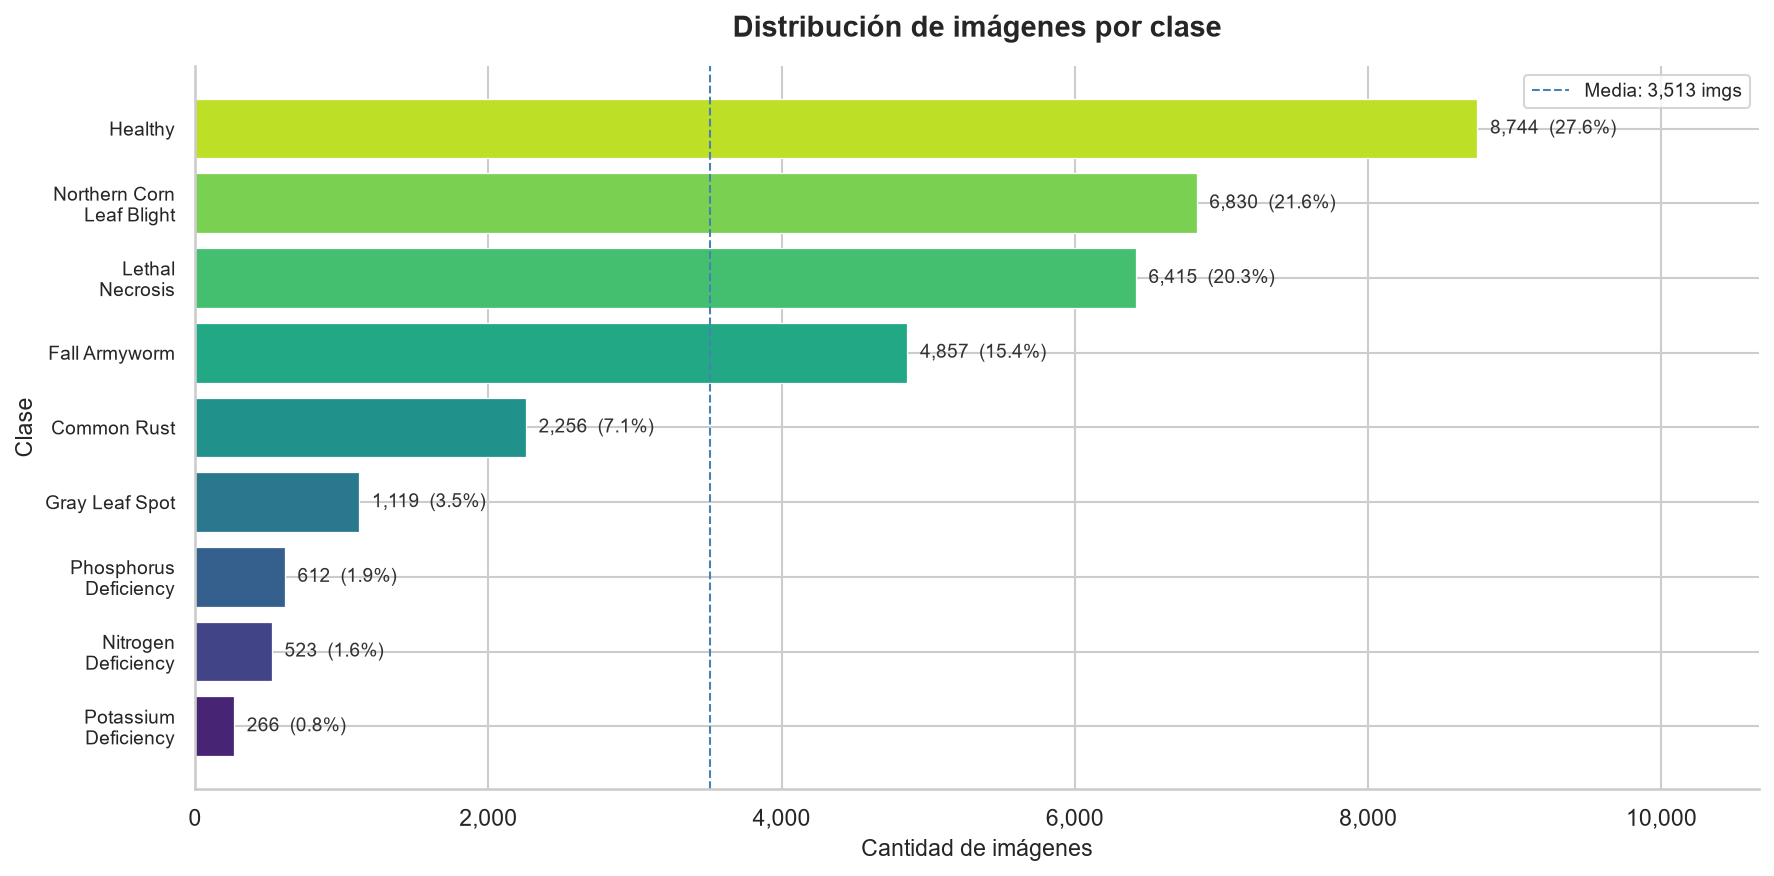
\includegraphics[width=0.95\linewidth]{images/eda/eda_01_distribucion_clases.png}
\caption{Distribuci\'on de im\'agenes por clase en \texttt{clean/}.}
\label{fig:dist}
\end{figure}

\textbf{Sesgo de dominio laboratorio/campo.} La proporci\'on lab/real var\'ia dr\'asticamente entre clases (Figura~\ref{fig:labreal}); el caso m\'as cr\'itico es \texttt{common\_rust}, con \textbf{95.4\%} de sus im\'agenes en entorno controlado. Un modelo entrenado sin cuidado podr\'ia aprender el fondo de laboratorio en lugar del s\'intoma foliar.

\begin{figure}[H]
\centering
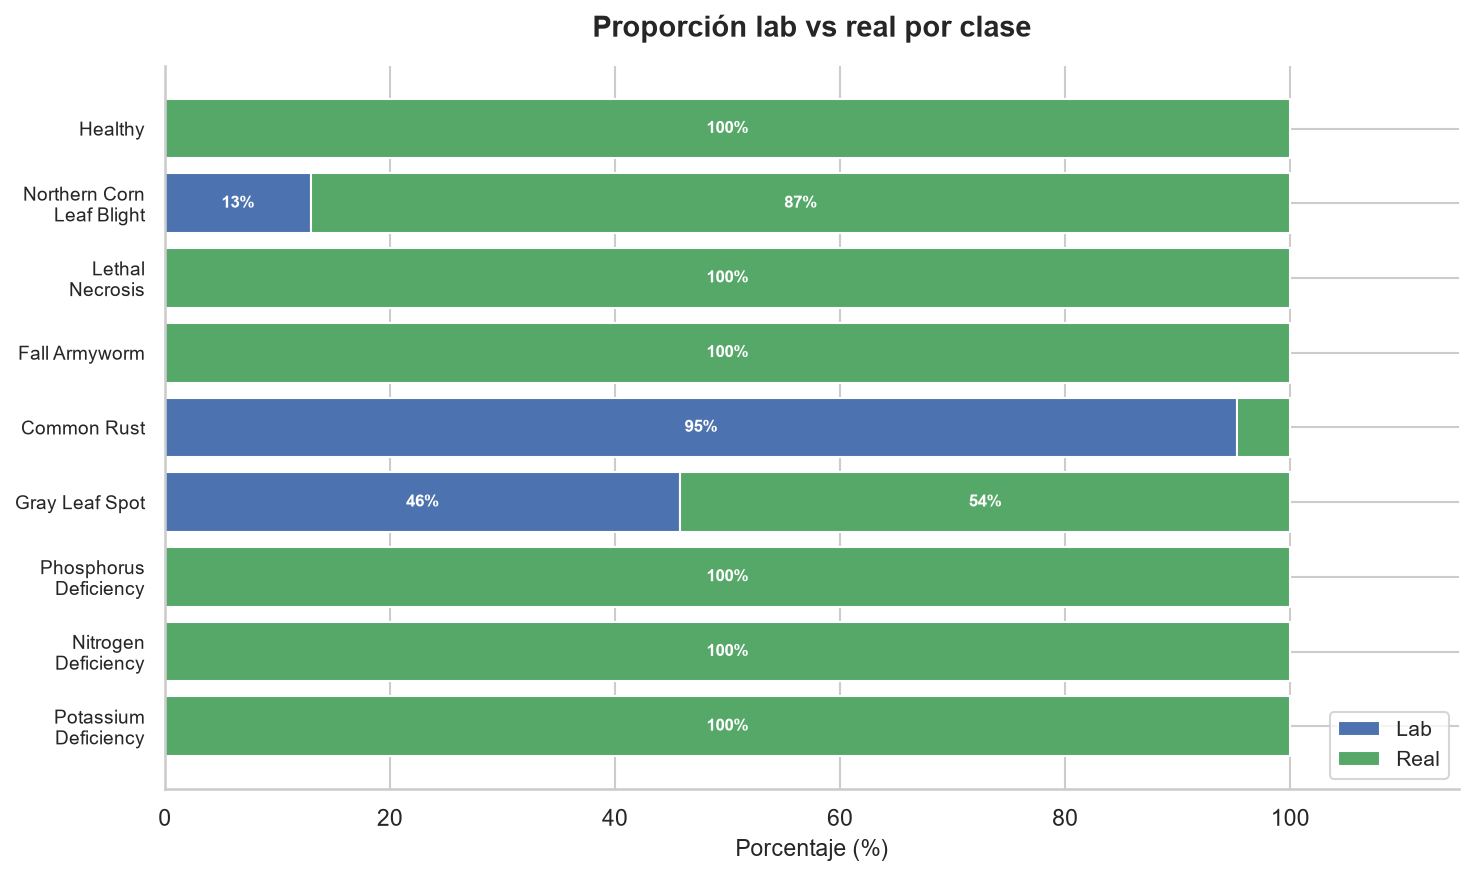
\includegraphics[width=0.95\linewidth]{images/eda/eda_02_lab_vs_real.png}
\caption{Proporci\'on de im\'agenes lab vs.\ real por clase.}
\label{fig:labreal}
\end{figure}

\textbf{Resoluci\'on heterog\'enea.} Las resoluciones var\'ian ampliamente entre fuentes (p.~ej.\ Roboflow ya redimensionado a 640$\times$640~px). El pipeline resuelve esto con \texttt{Resize} a la entrada del modelo (224$\times$224~px) como primera transformaci\'on.

\textbf{Calidad de imagen.} Sobre una muestra estratificada de hasta 400 im\'agenes por clase se evaluaron desenfoque (varianza del Laplaciano), sub- y sobre-exposici\'on; los problemas detectados son bajos y distribuidos uniformemente entre clases, por lo que no se aplic\'o ning\'un filtro autom\'atico de calidad.

\textbf{Sesgos combinados.} La Figura~\ref{fig:sesgos} resume cinco sesgos identificados: desbalance de clases, dominio de laboratorio, heterogeneidad visual intraclase, fuente \'unica en clases peque\~nas y concentraci\'on geogr\'afica. El sesgo de \texttt{fall\_armyworm} es cualitativo, no solo cuantitativo: mezcla dos se\~nales diagn\'osticas distintas seg\'un el dataset de origen -- hoja con da\~no sin insecto visible (\textit{corn\_leaf\_roboflow}, \textit{maize\_africa/Activity}) y hoja con da\~no y gusano visible (\textit{maize\_africa/Pest}, \textit{multicrop}) -- lo que puede llevar al modelo a aprender el insecto como atajo en lugar del patr\'on de da\~no foliar.

\begin{figure}[H]
\centering
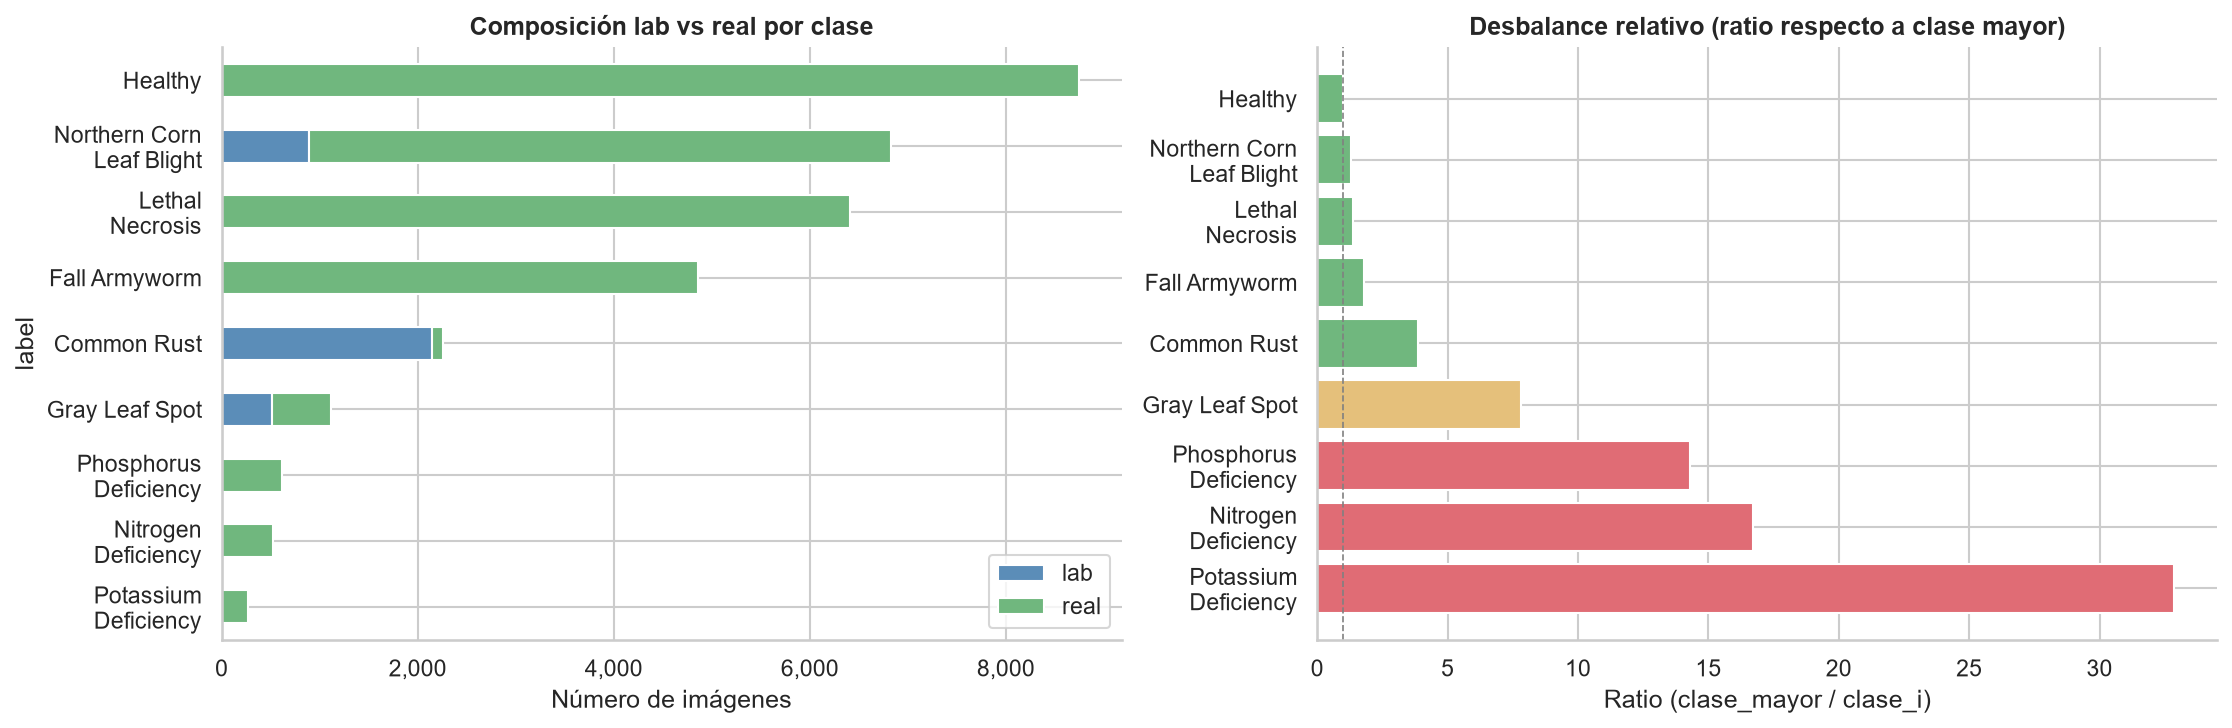
\includegraphics[width=0.95\linewidth]{images/eda/eda_06_sesgos.png}
\caption{Composici\'on lab/real y desbalance relativo por clase.}
\label{fig:sesgos}
\end{figure}

\section{Preprocesamiento y Feature Engineering}

Al tratarse de clasificaci\'on de im\'agenes con transfer learning, no existe ingenier\'ia de \textit{features} manual: las representaciones las aprende el backbone convolucional preentrenado en ImageNet. El esfuerzo de esta etapa se concentr\'o en normalizaci\'on, divisi\'on de datos y balanceo.

\subsection{Normalizaci\'on y divisi\'on de datos}

\textbf{Normalizado.} Todo tensor de imagen pasa por un \'unico punto de entrada (\texttt{load\_and\_normalize\_image()}): correcci\'on EXIF de orientaci\'on, conversi\'on a RGB estricta (descarta canal alfa, expande escalas de grises) y normalizaci\'on con media/desviaci\'on est\'andar de ImageNet ($\mu=[0.485,0.456,0.406]$, $\sigma=[0.229,0.224,0.225]$), requerida por los backbones preentrenados.

\textbf{Divisi\'on.} Estratificaci\'on jer\'arquica 70/15/15 (train/val/test) por \texttt{label + environment}, con semilla fija (42), para que la proporci\'on lab/real sea consistente en los tres conjuntos.

\subsection{Estrategia de balanceo}

El balanceo opera en tres capas complementarias: (1)~un tope configurable de im\'agenes por clase (1~500 en el perfil baseline) que recorta \'unicamente las clases mayoritarias, dejando intactas las minoritarias; (2)~\texttt{WeightedRandomSampler}, que asigna a cada muestra un peso $1/n_c$ ($n_c$ = frecuencia de su clase), igualando la frecuencia efectiva por \'epoca sin duplicar archivos; (3)~augmentation extendido (\texttt{CornMinorityTransforms}) \'unicamente para clases con ratio de desbalance $>4\times$: \texttt{RandomResizedCrop}, rotaci\'on aleatoria de hasta $\pm30^\circ$ (vs.\ $\pm15^\circ$ del pipeline est\'andar), \texttt{ColorJitter} m\'as agresivo y \texttt{GaussianBlur} suave, manteniendo el canal de matiz (\textit{hue}) casi intacto porque el diagn\'ostico de deficiencias nutricionales depende del color de la hoja. La funci\'on de p\'erdida (\texttt{CrossEntropyLoss}) se deja deliberadamente \textbf{sin ponderar}: ponderar sampler, augmentation y p\'erdida a la vez sobre-compensar\'ia el mismo desbalance por tres mecanismos distintos. Validaci\'on y prueba usan \'unicamente \texttt{Resize} + normalizaci\'on, sin aleatoriedad, para una evaluaci\'on determinista.

\section{Modelos Baseline}

Los \textit{baselines} de esta etapa cumplen dos prop\'ositos: (1) fijar un piso m\'inimo de comparaci\'on que arquitecturas m\'as complejas deber\'an superar consistentemente, y (2) permitir observar a bajo costo computacional el comportamiento inicial de cada arquitectura candidata (colapso de clases, sobreajuste temprano, incompatibilidades) antes de comprometer un entrenamiento completo.

\subsection{Dataset usado}

Los baselines se entrenan sobre el perfil \texttt{baseline} de la configuraci\'on del pipeline: las \textbf{9 clases} del dataset con un tope de \textbf{1~500 im\'agenes por clase}. Solo se recortan las clases mayoritarias; las minoritarias quedan intactas (potasio: 266, nitr\'ogeno: 523, f\'osforo: 612). Esto produce un dataset reducido de \textbf{10~020 im\'agenes} que conserva el desbalance natural de las clases peque\~nas (Tabla~\ref{tab:baselinesplit}).

\begin{table}[H]
\caption{Composici\'on del dataset baseline (9 clases, cap 1~500/clase)}
\label{tab:baselinesplit}
\centering
\small
\begin{singlespace}
\begin{tabular}{lr}
\toprule
\textbf{Split} & \textbf{Im\'agenes} \\
\midrule
Entrenamiento (70\%) & 7~014 \\
Validaci\'on (15\%) & 1~503 \\
Prueba (15\%) & 1~503 \\
\midrule
\textbf{Total} & \textbf{10~020} \\
\bottomrule
\end{tabular}
\end{singlespace}
\end{table}

El conjunto de prueba es mayoritariamente de \textbf{dominio real de campo} (1~182 im\'agenes reales vs.\ 321 de laboratorio), lo que permite medir el desempe\~no sobre fotos tomadas en condiciones agr\'icolas. Se usa la misma semilla (42) y estratificaci\'on \texttt{label+environment} que el dataset completo, para reproducibilidad.

\subsection{Arquitecturas seleccionadas}

Se priorizaron tres redes convolucionales ligeras preentrenadas en ImageNet con n\'umero de par\'ametros comparable, de modo que las diferencias de desempe\~no sean atribuibles a la arquitectura y no al tama\~no (Tabla~\ref{tab:models}). En los tres casos se reemplaza \'unicamente la capa clasificadora final por una capa lineal con el n\'umero de clases del proyecto, dejando el resto del backbone entrenable (\textit{fine-tuning} completo).

\begin{table}[H]
\caption{Arquitecturas baseline comparadas}
\label{tab:models}
\centering
\small
\begin{singlespace}
\begin{tabular}{lrrl}
\toprule
\textbf{Modelo} & \textbf{Par\'am.} & \textbf{Top-1 IN} & \textbf{Latencia rel.} \\
\midrule
EfficientNet-B0 & 5.3 M & $\sim$77.1\% & $\bigstar\bigstar$ \\
EfficientNet-Lite0 & 4.7 M & $\sim$74.9\% & $\bigstar\bigstar\bigstar$ \\
ShuffleNetV2-x1.0 & 2.3 M & $\sim$69.4\% & $\bigstar\bigstar\bigstar\bigstar$ (m\'as r\'apida) \\
\bottomrule
\end{tabular}
\end{singlespace}
\end{table}

\textbf{ShuffleNetV2-x1.0} (Ma et al., 2018) fue dise\~nada expl\'icitamente para inferencia eficiente en m\'oviles, usando operaciones de \textit{channel split} y \textit{channel shuffle} para esquivar el cuello de botella de memoria de convoluciones densas, resultando ser el modelo m\'as peque\~no de los evaluados ($\sim$5 MB serializado). \textbf{EfficientNet-B0} (Tan \& Le, 2019) usa bloques MBConv con SE integrado y es el punto de partida de la familia con \textit{compound scaling}. \textbf{EfficientNet-Lite0} es una variante de B0 sin bloques SE y con ReLU6 en lugar de Swish, dise\~nada expl\'icitamente para cuantizarse a INT8 sin p\'erdida significativa de precisi\'on (Google Brain/TensorFlow Team, 2020).

Entrenamiento: 20 \'epocas, batch 32, tasa de aprendizaje $10^{-4}$, \textit{weight decay} $10^{-4}$, pesos preentrenados.

\section{Resultados y M\'etricas}

\subsection{Resultados globales}

La Tabla~\ref{tab:results} resume el desempe\~no en prueba de los tres modelos sobre las 9 clases del dataset baseline (1~503 im\'agenes de prueba). La m\'etrica primaria es \textbf{macro-F1}, que pondera por igual todas las clases incluidas las minoritarias; accuracy es secundaria por el desbalance.

\begin{table}[H]
\caption{Comparaci\'on de modelos baseline en el conjunto de prueba (1~503 im\'agenes, 9 clases)}
\label{tab:results}
\centering
\begin{singlespace}
\begin{tabular}{lrrrr}
\toprule
\textbf{Modelo} & \textbf{Accuracy} & \textbf{macro-F1} & \textbf{Loss (test)} & \textbf{Checkpoint} \\
\midrule
EfficientNet-B0 & 0.9521 & \textbf{0.9146} & 0.229 & 15.6 MB \\
ShuffleNetV2-x1.0 & 0.9508 & 0.9030 & \textbf{0.169} & \textbf{5.0 MB} \\
EfficientNet-Lite0 & 0.9474 & 0.8951 & 0.218 & 13.1 MB \\
\bottomrule
\end{tabular}
\end{singlespace}
\end{table}

Los tres modelos superan la meta de macro-F1 $\geq0.85$ con holgura. EfficientNet-B0 lidera el macro-F1, pero la diferencia entre los tres es de apenas 2 puntos (0.9146 vs.\ 0.9030 vs.\ 0.8951), lo que los hace esencialmente equivalentes en calidad de clasificaci\'on para un test de 1~503 im\'agenes. ShuffleNetV2-x1.0 obtiene la menor loss de test (0.169) y el checkpoint m\'as peque\~no con diferencia (5~MB, $\sim$3$\times$ m\'as liviano que B0).

La Figura~\ref{fig:convergencia} muestra las curvas de convergencia durante el entrenamiento, donde se observa que los tres modelos alcanzan estabilidad en loss y macro-F1 de validaci\'on antes de la \'epoca~20.

\begin{figure}[H]
\centering
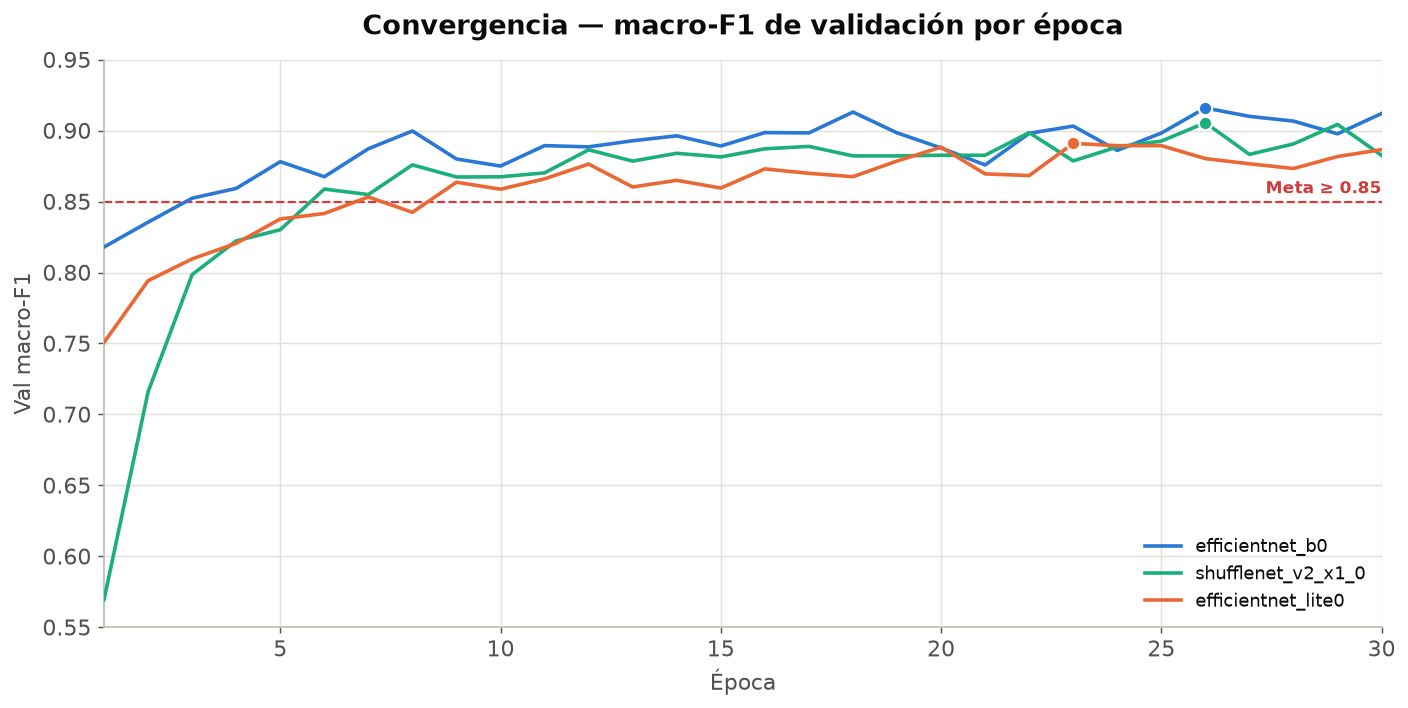
\includegraphics[width=0.95\linewidth]{images/baselines/baseline_convergencia.png}
\caption{Curvas de convergencia (loss y macro-F1) durante el entrenamiento de los tres baselines.}
\label{fig:convergencia}
\end{figure}

\subsection{F1 por clase}

La cifra agregada esconde que el rendimiento no es parejo entre clases. La Figura~\ref{fig:f1clase} y la Tabla~\ref{tab:f1clase} desglosan el F1 por clase y por modelo. El patr\'on es id\'entico en los tres: un bloque de clases ``f\'aciles'' que rozan o superan 0.95, un escal\'on intermedio en las lesiones foliares y las deficiencias de N y P, y una \'unica clase que se desploma por debajo de la meta: \texttt{potassium\_deficiency}.

\begin{figure}[H]
\centering
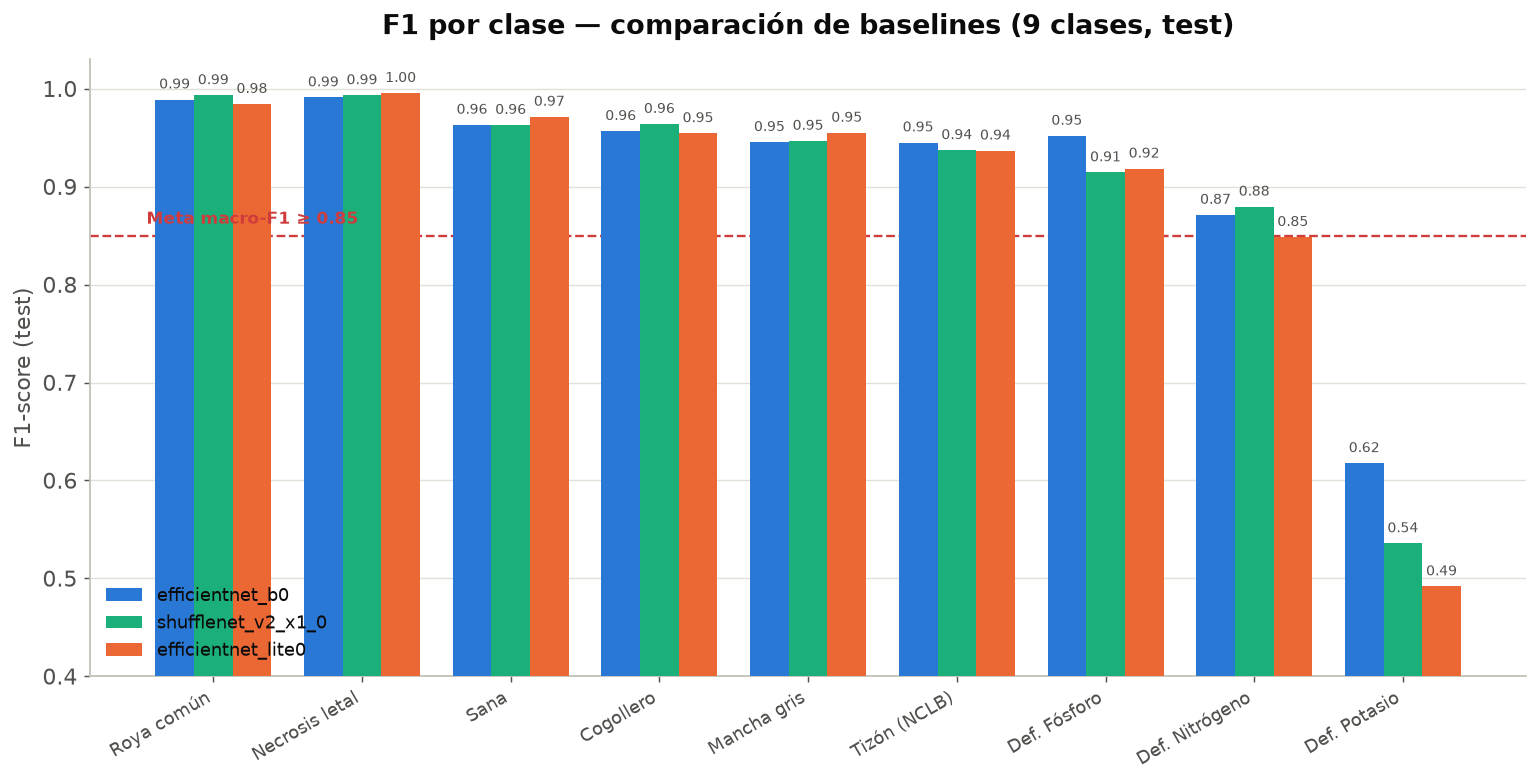
\includegraphics[width=0.95\linewidth]{images/baselines/baseline_f1_por_clase.png}
\caption{F1 por clase para los tres baselines, ordenado de mayor a menor.}
\label{fig:f1clase}
\end{figure}

\begin{table}[H]
\caption{F1 por clase y soporte en el conjunto de prueba}
\label{tab:f1clase}
\centering
\small
\begin{singlespace}
\begin{tabular}{lrrrr}
\toprule
\textbf{Clase} & \textbf{B0} & \textbf{ShuffleNet} & \textbf{Lite0} & \textbf{Soporte} \\
\midrule
common\_rust & 0.99 & 0.99 & 0.98 & 225 \\
lethal\_necrosis & 0.99 & 0.99 & 1.00 & 225 \\
healthy & 0.96 & 0.96 & 0.97 & 225 \\
fall\_armyworm & 0.96 & 0.96 & 0.95 & 225 \\
gray\_leaf\_spot & 0.95 & 0.95 & 0.95 & 168 \\
northern\_corn\_leaf\_blight & 0.95 & 0.94 & 0.94 & 224 \\
phosphorus\_deficiency & 0.95 & 0.92 & 0.92 & 92 \\
nitrogen\_deficiency & 0.87 & 0.88 & 0.85 & 79 \\
\textbf{potassium\_deficiency} & \textbf{0.62} & \textbf{0.54} & \textbf{0.49} & \textbf{40} \\
\bottomrule
\end{tabular}
\end{singlespace}
\end{table}

\subsection{El costo real de una sola clase}

Vale la pena cuantificar cu\'anto pesa \texttt{potassium\_deficiency} sobre la m\'etrica global. Si se recalcula el macro-F1 excluyendo esa \'unica clase, los tres modelos saltan a un rango estrecho y alto (Tabla~\ref{tab:sinpotasio}).

\begin{table}[H]
\caption{Impacto de \texttt{potassium\_deficiency} en el macro-F1 global}
\label{tab:sinpotasio}
\centering
\begin{singlespace}
\begin{tabular}{lrrr}
\toprule
\textbf{Modelo} & \textbf{macro-F1 (9 clases)} & \textbf{macro-F1 (sin potasio)} & \textbf{$\Delta$} \\
\midrule
EfficientNet-B0 & 0.9146 & \textbf{0.9517} & +0.037 \\
ShuffleNetV2-x1.0 & 0.9030 & 0.9490 & +0.046 \\
EfficientNet-Lite0 & 0.8951 & 0.9455 & +0.050 \\
\bottomrule
\end{tabular}
\end{singlespace}
\end{table}

Una sola clase minoritaria arrastra el macro-F1 global entre 3.7 y 5.0 puntos. El resto del clasificador ya opera a un nivel de $\sim$0.95 macro-F1. Esto reencuadra el problema: el baseline no necesita m\'as capacidad de modelo, sino resolver un cuello de botella de datos muy localizado.

\subsection{An\'alisis de confusi\'on}

La matriz de confusi\'on de EfficientNet-B0 (Figura~\ref{fig:confusion}), normalizada por fila (recall de cada clase real), hace visible que los errores no son ruido aleatorio sino que se agrupan en dos cl\'usteres.

\begin{figure}[H]
\centering
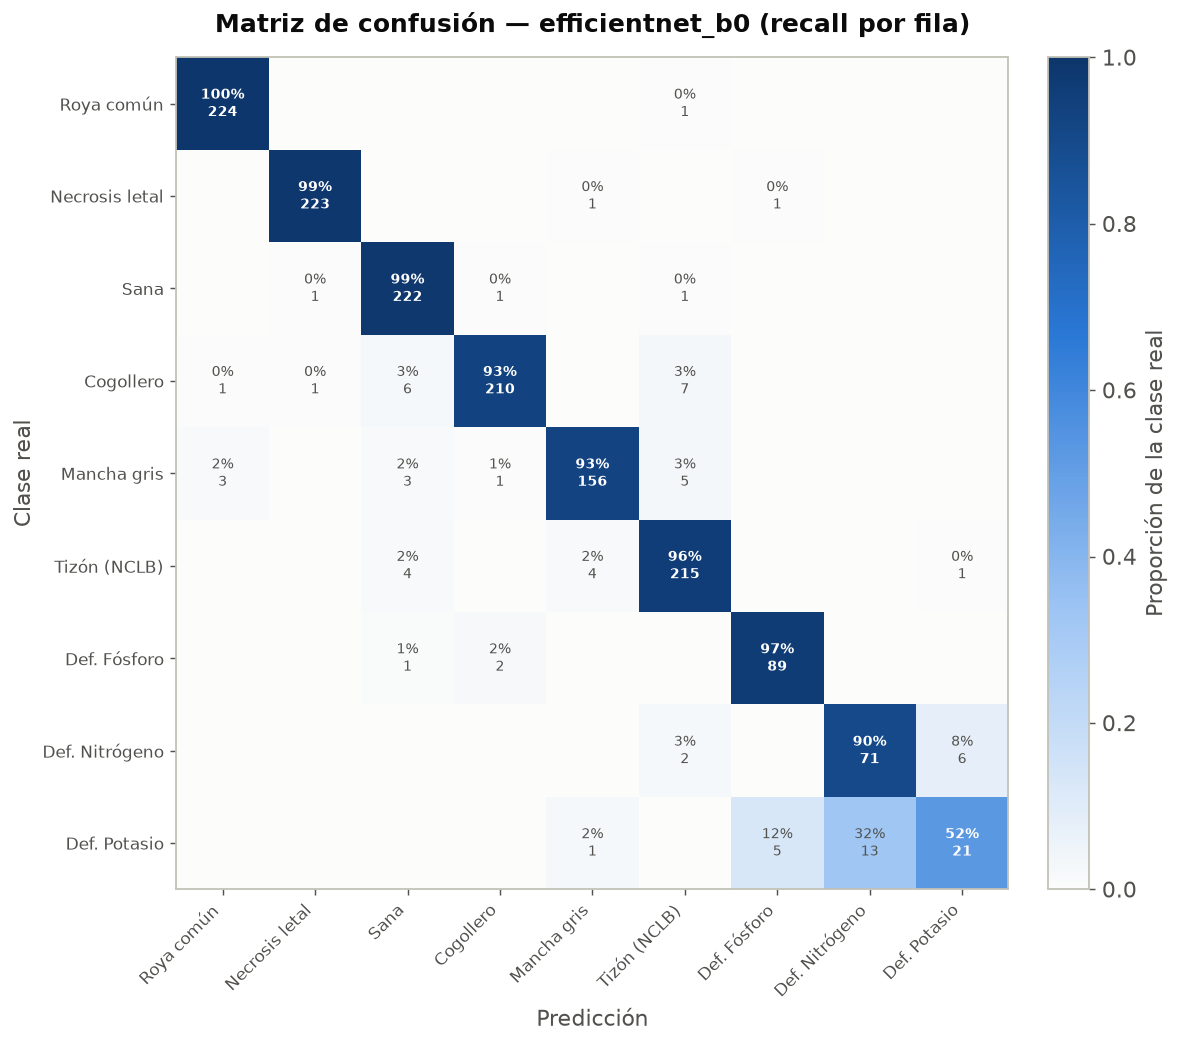
\includegraphics[width=0.85\linewidth]{images/baselines/baseline_confusion_b0.png}
\caption{Matriz de confusi\'on normalizada de EfficientNet-B0 (9 clases, test).}
\label{fig:confusion}
\end{figure}

\textbf{Cl\'uster 1 -- Deficiencias nutricionales (N/P/K).} El bloque inferior-derecho de la matriz concentra casi todo el error del modelo. De las 40 im\'agenes de potasio en test, solo 21 se clasifican correctamente; 13 se confunden con nitr\'ogeno y 5 con f\'osforo. La observaci\'on clave es que este error es \textit{dirigido}: si se toman todas las predicciones de las tres deficiencias juntas, el 97\% permanece dentro del propio cl\'uster N/P/K (solo 6 de 211 se escapan a una clase no nutricional). El modelo \textit{sabe} que est\'a viendo una deficiencia; lo que no logra es discriminar cu\'al de las tres, porque comparten el mismo s\'intoma base de clorosis y potasio es la clase con menos ejemplos de todo el dataset (266 im\'agenes totales).

\textbf{Cl\'uster 2 -- Lesiones foliares (GLS $\leftrightarrow$ NCLB).} \texttt{gray\_leaf\_spot} y \texttt{northern\_corn\_leaf\_blight} se confunden mutuamente (4--5 im\'agenes en cada sentido para B0) porque sus lesiones alargadas gris\'aceas/marrones son visualmente muy parecidas. Es un error de menor magnitud pero tambi\'en consistente entre los tres modelos.

Fuera de esos dos cl\'usteres, la matriz es pr\'acticamente diagonal: \texttt{common\_rust}, \texttt{lethal\_necrosis} y \texttt{healthy} se clasifican con recall $\geq0.99$.

\section{Interpretabilidad}

Se emple\'o LIME (\textit{Local Interpretable Model-agnostic Explanations}) (Ribeiro et al., 2016), que aproxima localmente el modelo de caja negra con un modelo lineal simple entrenado sobre perturbaciones de superp\'ixeles de la imagen de entrada, para revelar qu\'e regiones de la imagen influyen m\'as en la predicci\'on. El an\'alisis es post-hoc: no se acopla al ciclo de entrenamiento y se ejecuta bajo demanda sobre un modelo ya entrenado.

En los casos correctamente clasificados (p.~ej.\ Figura~\ref{fig:lime_correct}, \texttt{healthy} en campo real), LIME resalta consistentemente segmentos sobre el tejido foliar y no sobre el fondo, indicio de que el modelo no depende de atajos de fondo en estos ejemplos.

\begin{figure}[H]
\centering
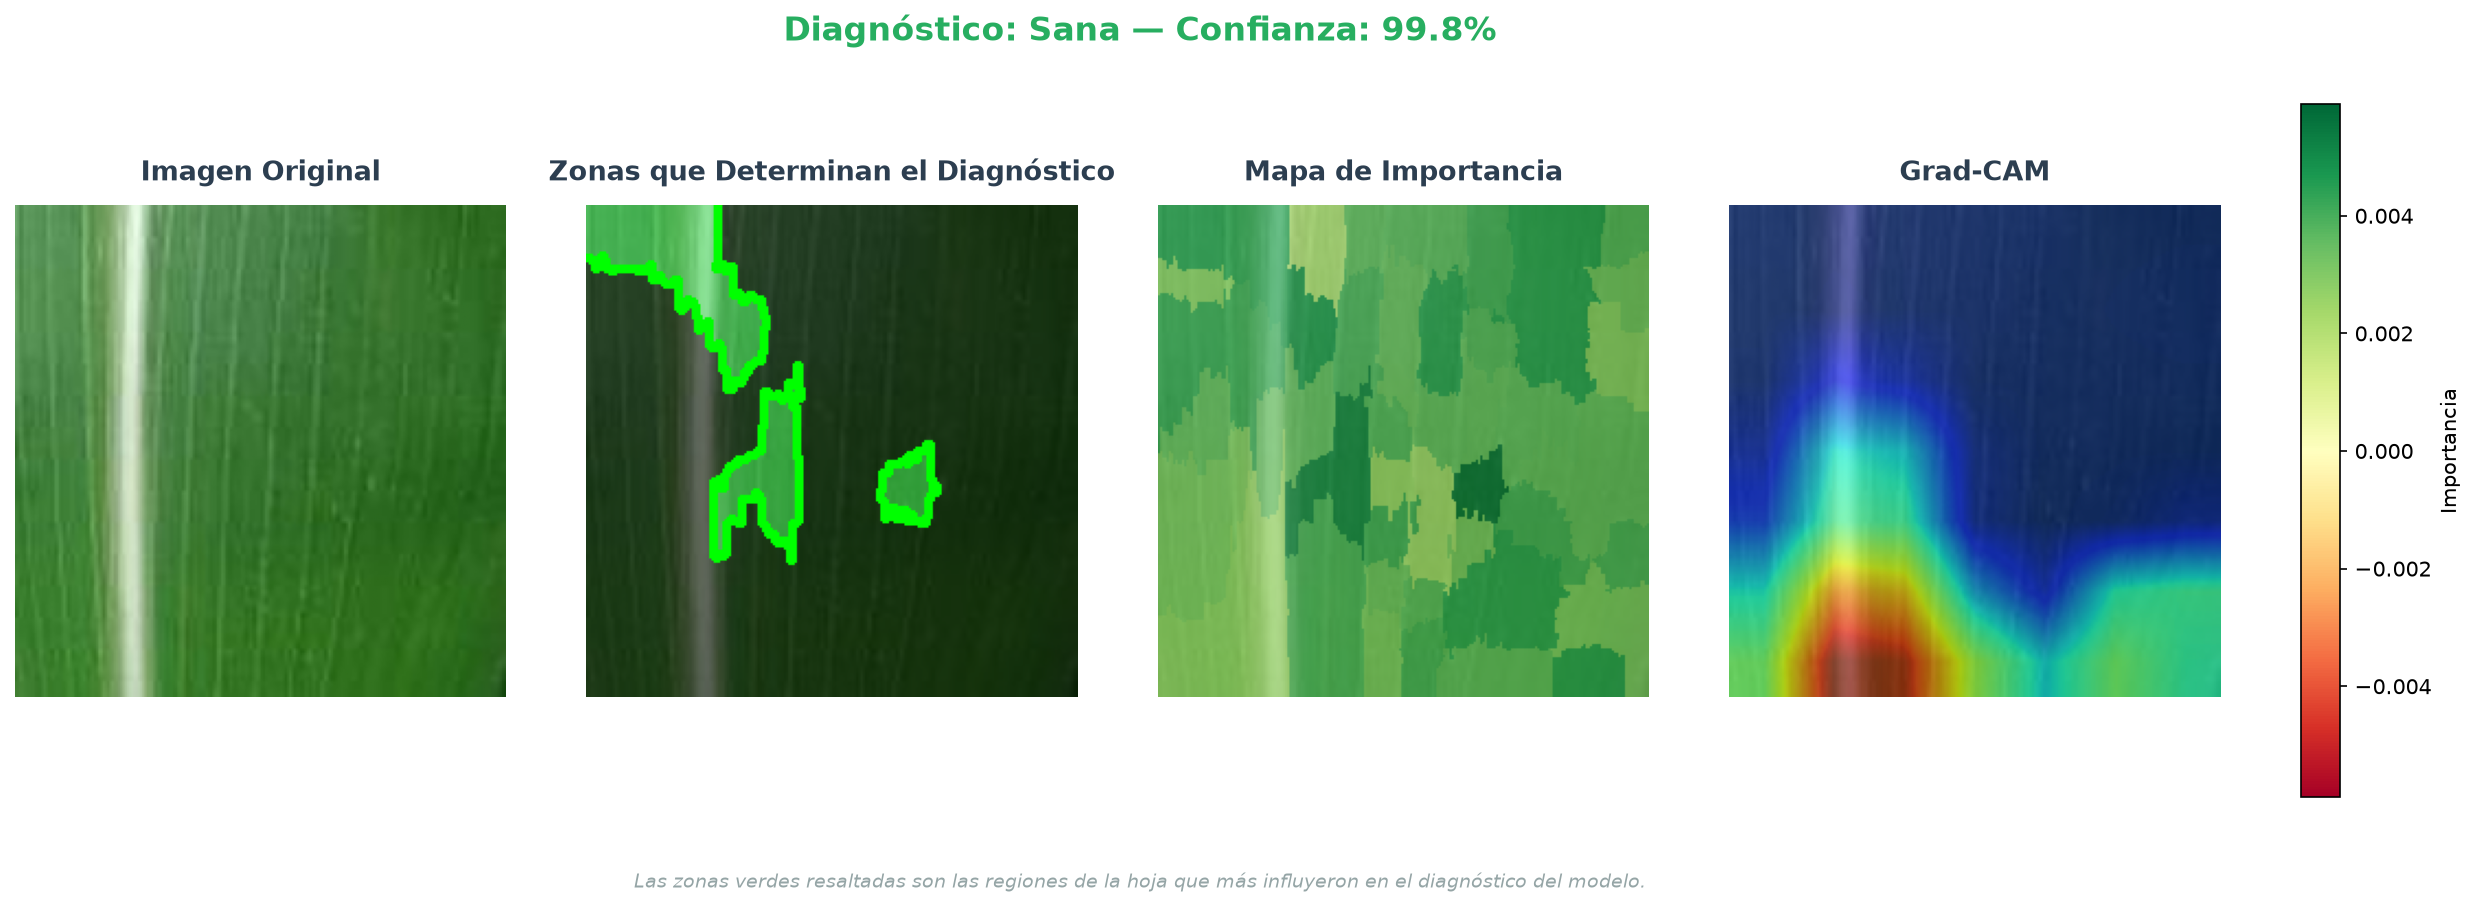
\includegraphics[width=0.85\linewidth]{images/lime/shufflenet_v2_x1_0_healthy_correct.png}
\caption{Explicaci\'on LIME de un acierto de ShuffleNetV2-x1.0 (\texttt{healthy}, campo real).}
\label{fig:lime_correct}
\end{figure}

Adicionalmente, la Figura~\ref{fig:lime_nitrogen} muestra un caso de EfficientNet-B0 sobre la clase \texttt{nitrogen\_deficiency} (campo real), correctamente diagnosticada con 99.99\% de confianza. LIME evidencia c\'omo el modelo concentra su atenci\'on en el patr\'on de decoloraci\'on caracter\'istico (clorosis) de la hoja, demostrando que la red ha aprendido las se\~nales agron\'omicas clave de la deficiencia nutricional y no solo atajos del fondo.

\begin{figure}[H]
\centering
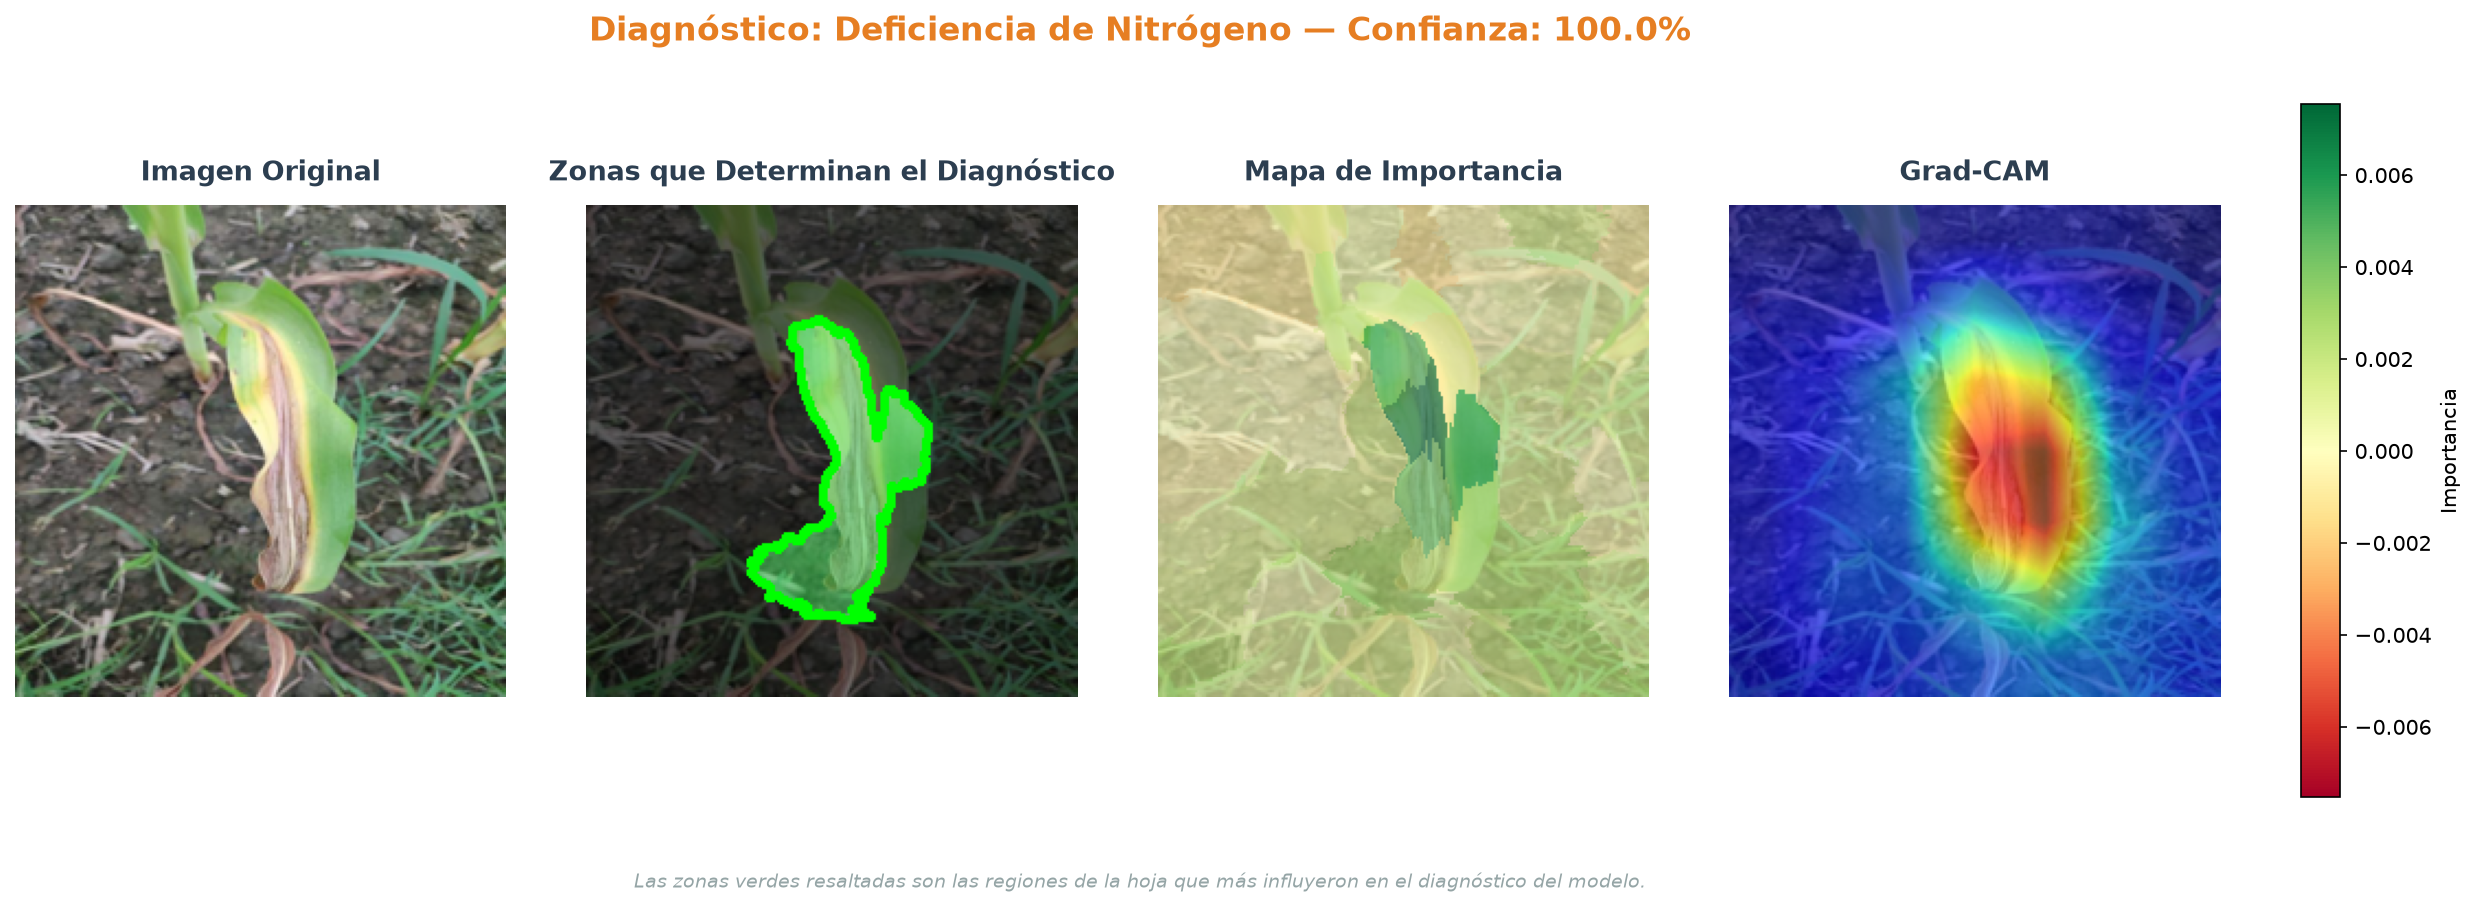
\includegraphics[width=0.85\linewidth]{images/lime/b0_nitrogen_correct.png}
\caption{Explicaci\'on LIME de un acierto de EfficientNet-B0 en deficiencia nutricional (\texttt{nitrogen\_deficiency}, campo real, 99.99\% de confianza).}
\label{fig:lime_nitrogen}
\end{figure}

La Figura~\ref{fig:lime_error} muestra un caso de error real de EfficientNet-Lite0: una imagen de \texttt{nitrogen\_deficiency} (campo real) clasificada como \texttt{fall\_armyworm}. LIME permite inspeccionar visualmente si el error proviene de una textura foliar ambigua o de una se\~nal espuria del entorno, en lugar de quedarse \'unicamente con el n\'umero agregado de la matriz de confusi\'on.

\begin{figure}[H]
\centering
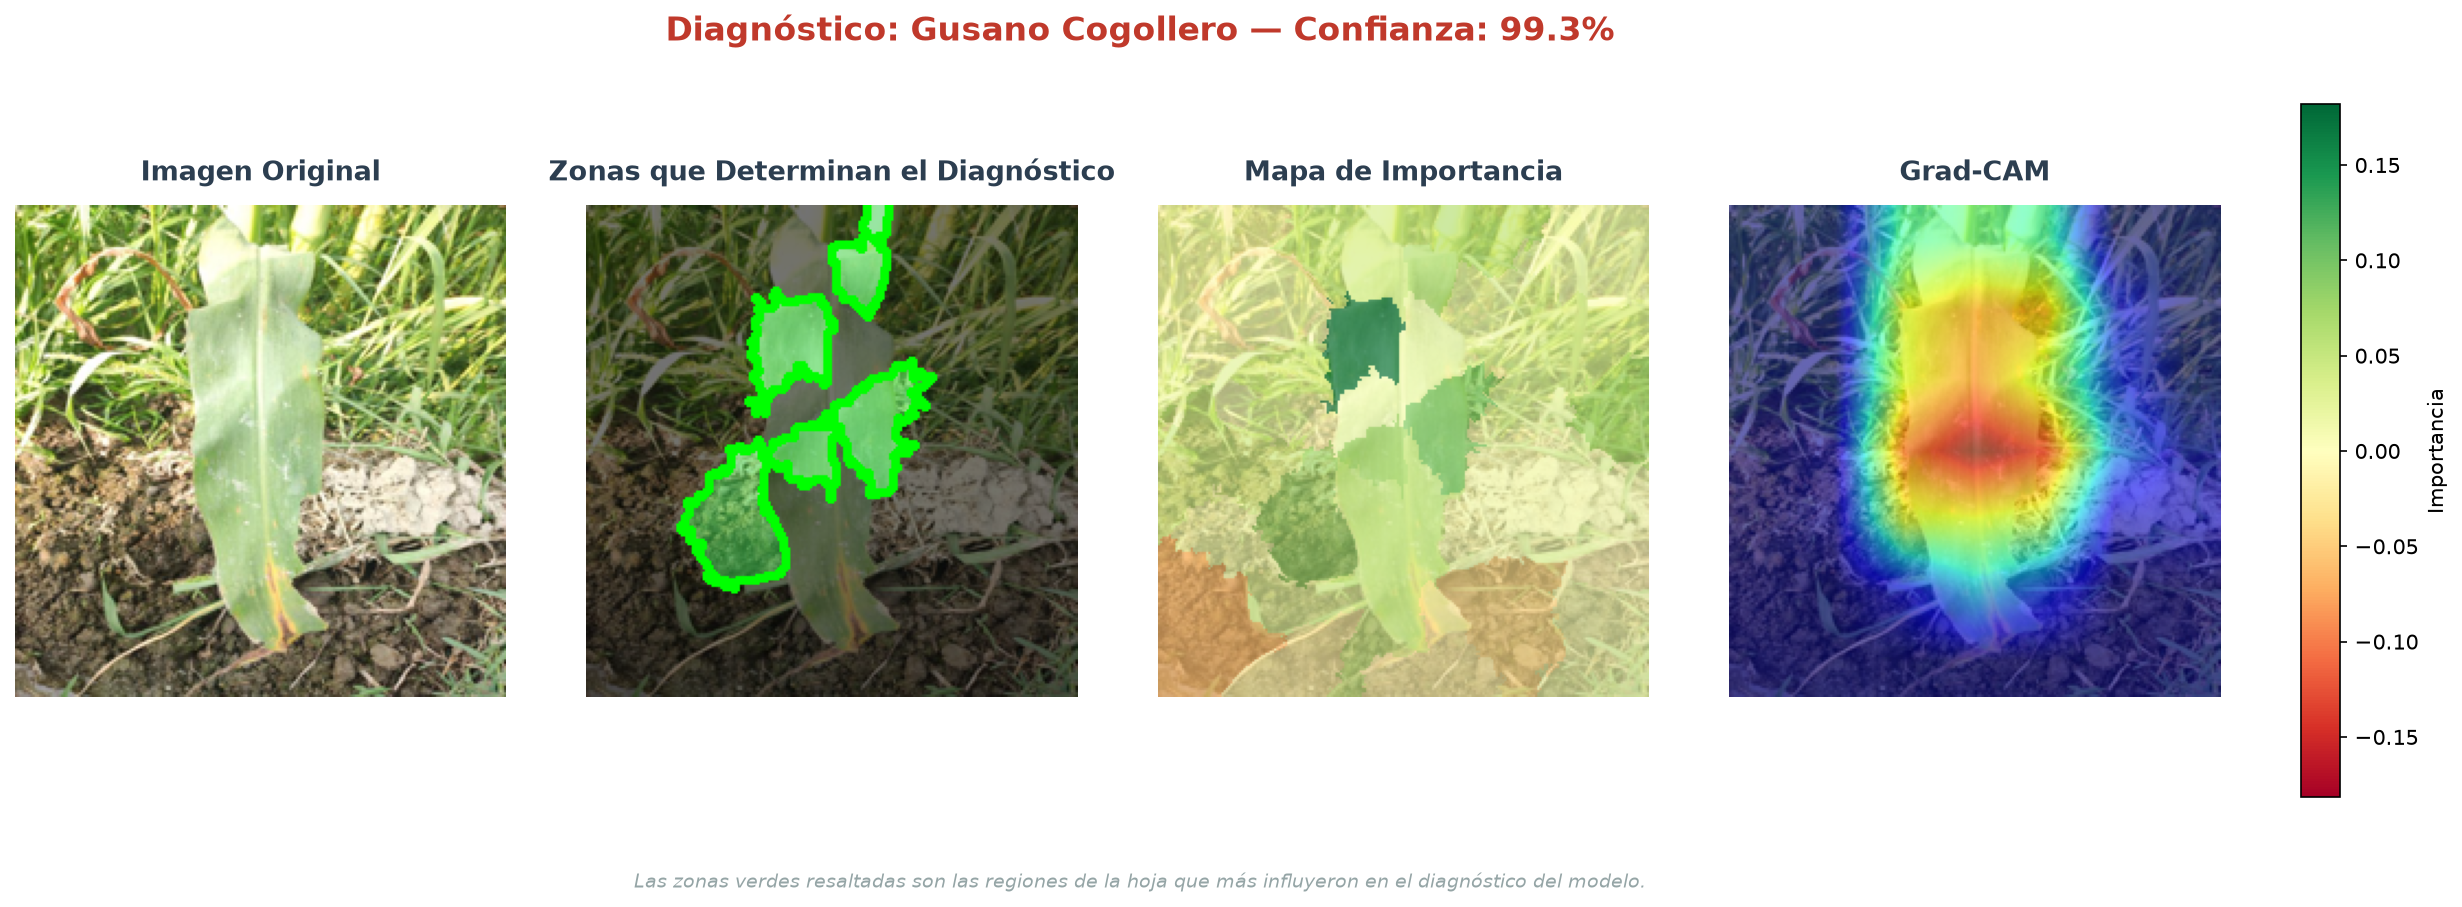
\includegraphics[width=0.85\linewidth]{images/lime/efficientnet_lite0_nitrogen_error.png}
\caption{Explicaci\'on LIME de un error real de EfficientNet-Lite0 (\texttt{nitrogen\_deficiency} clasificada como \texttt{fall\_armyworm}).}
\label{fig:lime_error}
\end{figure}

\textit{Nota:} las im\'agenes LIME presentadas corresponden a una corrida preliminar de 4 clases; sirven como ejemplo cualitativo del tipo de an\'alisis que LIME habilita. Un an\'alisis de interpretabilidad sistem\'atico sobre las 9 clases --- incluyendo fidelidad agregada y auditor\'ia de estabilidad de LIME --- es parte del trabajo futuro.

\section{Conclusiones y Trabajo Futuro}

Sobre las 9 clases del dataset con tope de 1~500 im\'agenes/clase, EfficientNet-B0 obtiene el mejor macro-F1 (0.9146), seguido de ShuffleNetV2-x1.0 (0.9030) y EfficientNet-Lite0 (0.8951). Los tres superan la meta de macro-F1 $\geq0.85$ y son esencialmente equivalentes en calidad de clasificaci\'on (diferencias de $\sim$2 puntos porcentuales).

El hallazgo m\'as relevante es que \texttt{potassium\_deficiency} es el \'unico cuello de botella que impide subir la m\'etrica global: con F1 de 0.49--0.62 y solo 40 im\'agenes en test, arrastra el macro-F1 entre 3.7 y 5.0 puntos. Excluyendo esa clase, los tres modelos operan a $\sim$0.95 macro-F1. El modelo ya detecta la categor\'ia ``deficiencia nutricional'' con alt\'isima fiabilidad (97\% de contenci\'on en el cl\'uster N/P/K), pero no logra discriminar cu\'al de las tres por la escasez de datos de potasio.

Para la Etapa~2, las l\'ineas de trabajo prioritarias son:

\begin{itemize}
\item \textbf{M\'as datos de potasio.} Aumentar/rebalancear las deficiencias nutricionales (especialmente potasio) mediante recolecci\'on de im\'agenes reales adicionales, augmentation dirigido o p\'erdida ponderada por clase.
\item \textbf{An\'alisis de interpretabilidad sobre 9 clases.} Extender el an\'alisis LIME y Grad-CAM a las 9 clases con fidelidad agregada y auditor\'ia de estabilidad.
\item \textbf{Elecci\'on de arquitectura para despliegue.} Dado que los tres modelos son equivalentes en calidad, la decisi\'on final debe priorizar tama\~no y latencia en hardware objetivo, lo que por ahora favorece a ShuffleNetV2-x1.0 (5~MB, menor loss). Se requieren pruebas con el modelo exportado a TFLite en dispositivo real.
\item \textbf{Entrenamiento completo.} Entrenar sobre el dataset completo (31~623 im\'agenes) sin tope, con las estrategias de balanceo refinadas a partir de los hallazgos de esta etapa.
\end{itemize}

\section{Referencias}
\addcontentsline{toc}{section}{Referencias}

\noindent\hangindent=1.27cm\hangafter=1
Google Brain / TensorFlow Team. (2020, marzo). \textit{Higher accuracy on vision models with EfficientNet-Lite}. TensorFlow Blog. \url{https://blog.tensorflow.org/2020/03/higher-accuracy-on-vision-models-with-efficientnet-lite.html}

\par\bigskip
\noindent\hangindent=1.27cm\hangafter=1
Ma, N., Zhang, X., Zheng, H.-T., \& Sun, J. (2018). ShuffleNet V2: Practical guidelines for efficient CNN architecture design. En \textit{Proceedings of the European Conference on Computer Vision (ECCV)} (pp. 116--131). Munich, Germany.

\par\bigskip
\noindent\hangindent=1.27cm\hangafter=1
Hu, J., Shen, L., \& Sun, G. (2018). Squeeze-and-excitation networks. En \textit{Proceedings of the IEEE/CVF Conference on Computer Vision and Pattern Recognition (CVPR)} (pp. 7132--7141). Salt Lake City, UT, USA.

\par\bigskip
\noindent\hangindent=1.27cm\hangafter=1
Ribeiro, M. T., Singh, S., \& Guestrin, C. (2016). ``Why should I trust you?'': Explaining the predictions of any classifier. En \textit{Proceedings of the 22nd ACM SIGKDD International Conference on Knowledge Discovery and Data Mining (KDD)} (pp. 1135--1144). San Francisco, CA, USA.

\par\bigskip
\noindent\hangindent=1.27cm\hangafter=1
Tan, M., \& Le, Q. V. (2019). EfficientNet: Rethinking model scaling for convolutional neural networks. En \textit{Proceedings of the 36th International Conference on Machine Learning (ICML)} (pp. 6105--6114). Long Beach, CA, USA.

\end{document}
